\chapter{Planejamento do Experimento}\label{chapter:experimento}

Neste capítulo é apresentado o experimento que será realizado para a avaliação da proposta apresentada no Capítulo \ref{chapter:proposta}.
Para avaliar a proposta deste trabalho irá utilizar uma avaliação pela perspectiva do usuário, que segundo a definição de
\citeonline{shani2011evaluating} se encaixa em um Estudo com usuários. O algoritmo proposto será incorporado ao ambiente
AdaptWeb\textsuperscript e avaliado em uma situação real de uso em um minicurso de algoritmos. Esse capítulo explica
em mais detalhes o ambiente AdaptWeb\textsuperscript, as mudanças propostas para o ambiente e o experimento planejado.

\section{Descrição do Ambiente \adaptweb}

O \adaptweb (Ambiente de Ensino-Aprendizagem Adaptativo na Web) é um sistema open source
que consiste em um AVA capaz de adaptar o conteúdo, a apresentação e a navegação em determinado curso às características
e preferências do aluno \cite{gasparini2009adaptweb}. A Subseção \ref{subsection:estrutura-adaptweb} apresenta a Estrutura Geral do
\adaptweb.

\subsection{Estrutura do \adaptweb}\label{subsection:estrutura-adaptweb}

A estrutura do \adaptweb é composta por quatro módulos: (1) o módulo de autoria; (2) o
módulo de armazenamento em XML (Extensible Markup Language); (3) o módulo de adaptação do conteúdo baseado no modelo do
usuário e (4) o módulo de interface adaptativa \cite{gasparini2003interface}, conforme pode ser visto na Figura
\ref{fig:adaptweb-arquitetura}.

\begin{figure}[htb]
  \caption{\label{fig:adaptweb-arquitetura}Estrutura do \adaptweb}
  \begin{center}
      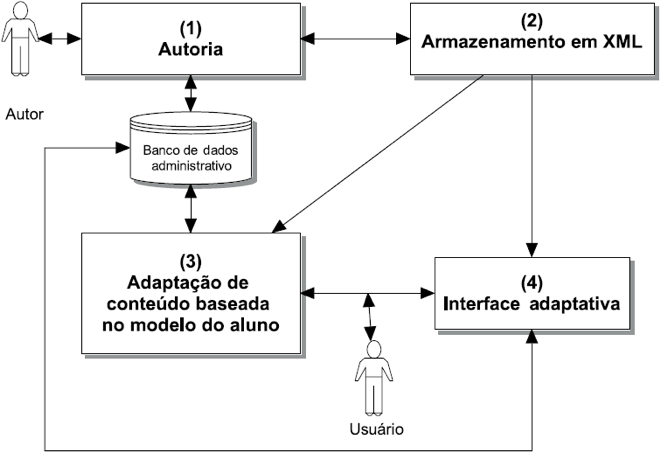
\includegraphics[scale=1.0]{./Figuras/adaptweb-arquitetura.png}
  \end{center}
  \legend{Fonte: \citeonline{gasparini2003interface}}
\end{figure}

O módulo de autoria (1) consiste na organização do conteúdo instrucional a ser disponibilizado para o aluno, sendo que
este conteúdo pode ter arquivos classificados como conceito, exemplos, exercícios e materiais complementares
\cite{gasparini2003interface}. Ao criar um conteúdo no sistema, o autor pode definir para quais cursos e disciplinas
deseja que o conteúdo ou arquivo esteja disponível. Isto significa que um aluno de um Curso X e de outro Curso Y,
matriculados em uma mesma disciplina, podem ter conteúdos distintos, conforme definido pelo professor. Por exemplo, a
disciplina de Cálculo I pode ser oferecida para os cursos de Ciência da Computação e Engenharia Elétrica e sua
abrangência e profundidade pode ser distinta para cada curso.

Em \citeonline{de2015sistema}, foi proposto uma nova categoria para os conteúdos chamada Links de Apoio. Esses Links de Apoio
são links externos ao ambiente \adaptweb que são cadastrados pelo professor como um
material alternativo de estudo e não estão diretamente atrelados á nenhum conceito em específico. O objetivo foi criar
uma nova categoria de materiais que poderia ser recomendada para o usuário a qualquer momento de sua interação.

O módulo de armazenamento em XML (2) é responsável por organizar os conteúdos e arquivos disponibilizados pelo autor em
um arquivo XML \cite{gasparini2003interface}. É utilizada a representação através de XML devido à sua alta
flexibilidade, oferecendo a estruturação dos documentos de forma independente da apresentação.

O módulo de adaptação do conteúdo baseado no modelo do aluno (3) é responsável por adaptar o conteúdo da disciplina
para cada curso. Por fim, o módulo de interface adaptativa (4) é responsável pela adaptação da navegação e da
apresentação da interface do ambiente de acordo com o curso, preferências do modo de navegação (modo tutorial ou livre)
e o conhecimento do usuário \cite{gasparini2003interface}.

\subsection{Sistema de Recomendação no \adaptweb}

Na Subseção \ref{subsection:estrutura-adaptweb} foi apresentada a estrutura do ambiente \adaptweb, que possui quatro categorias
de materiais para cada conteúdo. Além disso, existe uma outra categoria chamada Links de Apoio com o propósito de ser um
material auxiliar e que pode ser recomendado a qualquer momento para o usuário.

Fazendo uma relação da estrutura do \adaptweb com o algoritmo proposto no Capítulo \ref{chapter:proposta}, os itens de
das categorias Conceito, Materiais Complementares e os próprios Links de Apoio serão considerados para a composição do perfil do usuário. Todos os
materiais acessados em cada uma das categorias é representado através das palavras-chave, e
essas palavras-chave farão parte do perfil do aluno a partir do momento em que este acessar o material. Já para os itens
recomendados, apenas os Links de Apoio serão utilizados.

Como no ambiente \adaptweb as palavras-chave para o itens podem ser cadastradas pelo professor da disciplina, não será
utilizada nenhuma técnica para captura automática das palavras-chave. Para a representação dos materiais envolvidos no
processo de recomedanção (i.e., Conceitos, Materiais Complementares e Links de Apoio) foi criado um Dicionário de Palavras-Chave
com as possíveis palavras a ser utilizadas. Esse Dicionário foi essencial para o funcionamento do SR, pois garante que as
palavras-chave presentes nos materiais que são similares também serão similares. Isso evita a necessidade de lidar com palavras-chave
sinônimas ou a variação de singular e plural, já que as palavras-chave que podem ser utilizadas para representar os materiais
são restritas às presentes no dicionário.

O Dicionário completo pode ser visto no Apêndice \ref{ape:dicionario-palavras-chave}. A criação do Dicionário foi validado
por um aluno do Mestrado em Ensino de Ciências, Matemática e Tecnologias que também é professor da disciplina de
Algoritmos no SENAC-SC. O professor teve acesso ao Minicurso de Algoritmos utilizado no experimento
e teve o papel de avaliar o Dicionário criado e acrescentar mais palavras para agregar conjunto de palavras-chave.

Depois de criado e validado o Dicionário, foi realizada a associação de forma manual entre cada material dos Conceitos,
Materiais Complementares e Links de Apoio com as palavras-chave do Dicionário. No total, 51 Conceitos, 28 Materiais
Complementares e 108 Links de Apoio foram analisados. O resultado dessa associação pode ser visto no Apêndice \ref{ape:palavras-chave-materiais}.

O Sistema de Recomendação (SR) irá buscar, com base nos itens acessados pelo aluno, os Links de Apoio mais adequados
para a recomendação e irá apresentar através de uma lista de itens. A forma de apresentação das Recomendações é discutida
em mais detalhe na Subseção \ref{subsection:apresentacao-recomendacoes}.

\subsection{Apresentação das Recomendações}\label{subsection:apresentacao-recomendacoes}

A lista de recomendações neste trabalho será apresentada ao aluno na tela principal do ambiente do aluno. Dessa forma,
quando o SR possuir itens para recomendar para o usuário esses itens aparecem em uma lista logo abaixo do conteúdo que
ele estiver visualizando no momento, independente se o aluno estiver na tela de Conceito, Exercícios, Exemplos ou
Materiais Complementares. Na Figura \ref{fig:adaptweb-proposta-recomendacao} pode-se observar a tela inicial do ambiente do
aluno, onde estão destacadas as seguintes áreas: (1) Menu de navegação pelos tópicos; (2) Categorias dos materiais dentro
do ambiente; (3) Interface das recomendações; (4) Mapa da disciplina; (5) Ajuda. As recomendações podem ser apresentadas ao usuário no momento em que este estiver acessando
quaisquer itens que sejam da categoria Conceito e Materiais Complementares, assim que o SR possuir itens relevantes para recomendar.

\begin{figure}[htb]
  \caption{\label{fig:adaptweb-proposta-recomendacao}Proposta de Interface de Recomendação}
  \begin{center}
      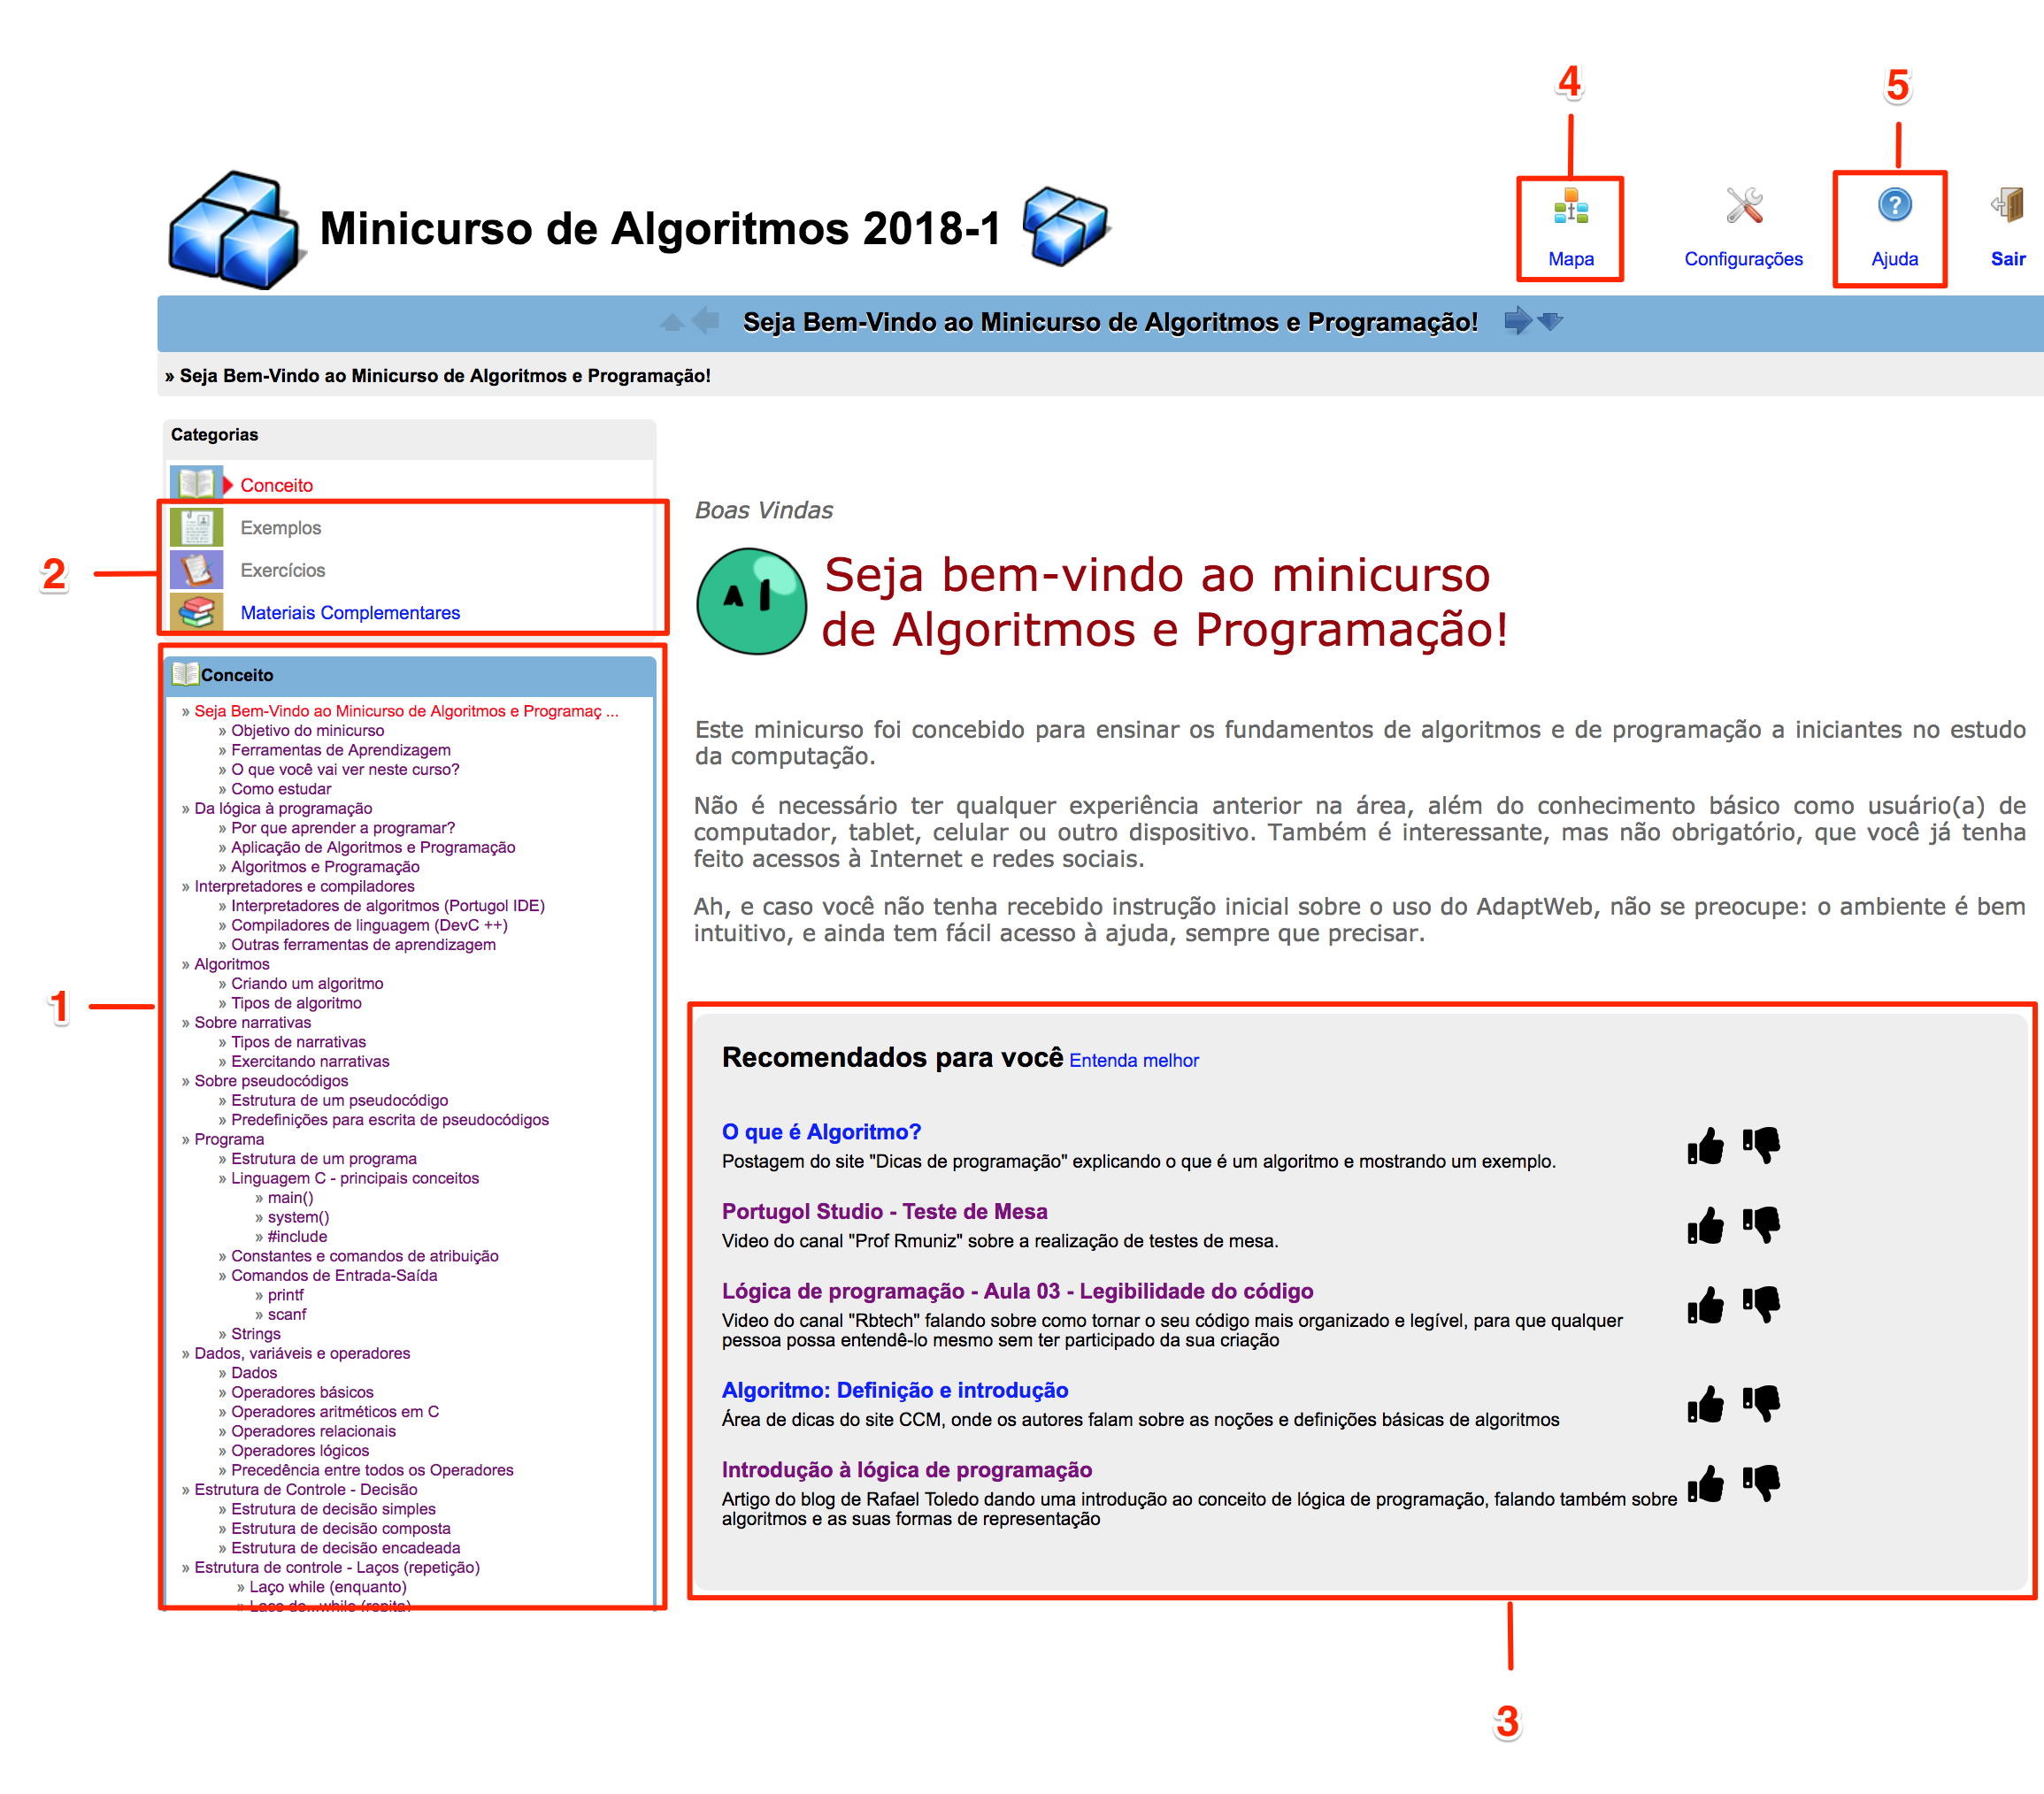
\includegraphics[scale=0.4]{./Figuras/interface-recomendacao.png}
  \end{center}
  \legend{Fonte: O autor.}
\end{figure}

Como visto na imagem, as principais informações dos Links de Apoio recomendados apresentados para o aluno são: Link, Nome do Link, Descrição e a possibilidade de avaliar o item
positivamente ou negativamente. A avaliação feita pelo usuário não é considerada pelo algoritmo de recomendação, sendo que os itens acessados pelo
usuário são considerados como do seu interesse. Como trabalho futuro é possível incorporar a avaliação na recomendação, e.g.,
não tornar a recomendar itens que foram avaliado com notas baixas ou apenas considerar para o algoritmo Baseado em Conteúdo
os itens avaliados positivamente. \citeonline{pu2012evaluating} afirmam que enquanto recomendar um item apenas é pouco, recomendar mais do que cinco itens
aumenta a dificuldade de escolhar do usuário. Por isso, a quantidade máxima de itens recomendadas para o usuário em cada
recomendação é de cinco itens.

Para cumprir o requisito de Explicação das recomendações citada por \citeonline{pu2012evaluating}, foi adicionado o
botão de "Entenda melhor" que tem por objetivo explicar ao usuário como a lista de itens foi gerada. Ao entender o
funcionamento do algoritmo de recomendação o usuário tem a possibilidade aprimorar o seu perfil para personalizar as
recomendações recebidas. Na Figura \ref{fig:adaptweb-proposta-explicacao} está um protótipo da explicação da recomendação
mostrada para o aluno.

\begin{figure}[htb]
  \caption{\label{fig:adaptweb-proposta-explicacao}Explicação da recomendação}
  \begin{center}
      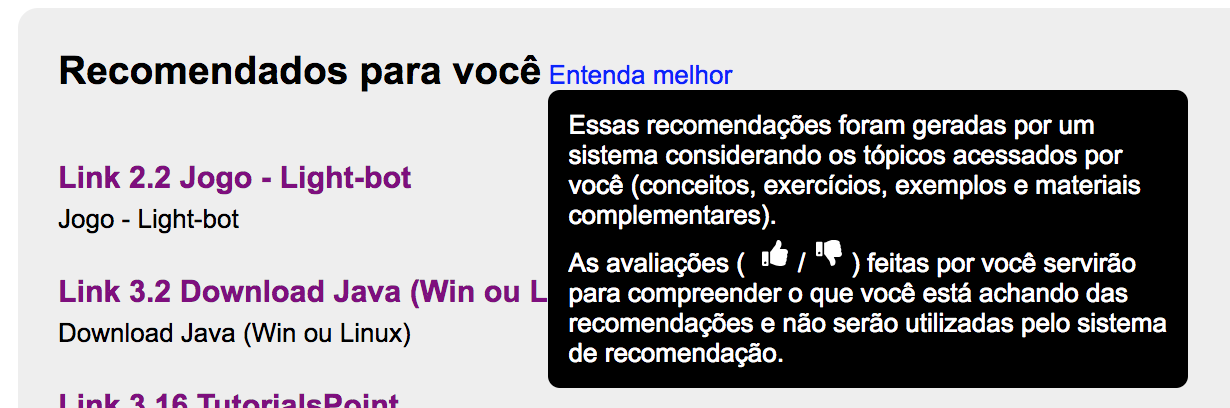
\includegraphics[scale=0.6]{./Figuras/explicacao-das-recomendacoes.png}
  \end{center}
  \legend{Fonte: O autor.}
\end{figure}

\section{Definição do experimento}

O experimento proposto neste trabalho visa avaliar a experiência dos alunos ao interagir com o SR proposto, se comparado a um SR
utilizando a abordagem Baseada em Conteúdo tradicional. Este experimento foi
baseado nas seguintes hipóteses:

\begin{itemize}
\item \textbf{H\textsubscript{0}:} Não há diferenças na percepção do usuário da qualidade das recomendações recebidas utilizando a abordagem
Baseada em Conteúdo tradicional e a proposta desse trabalho.
\item \textbf{H\textsubscript{1}:} Há diferenças na percepção do usuário da qualidade das recomendações recebidas utilizando a abordagem
Baseada em Conteúdo tradicional e a proposta desse trabalho.
\end{itemize}

Para a execução do experimento, o SR proposto foi comparado a abordagem Baseada em Conteúdo tradicional utilizando uma
estratégia \textit{Between Subjects}, i.e., os alunos serão divididos em dois grupos e cada grupo irá testar apenas
um dos sistemas. Para garantir que a única variável seja o SR utilizado, ambos os grupos irão utilizar a mesma
interface proposta para as recomendações.

O experimento foi realizado através do Minicurso de Algoritmos e Linguagem de Programação, o qual teve seu design instrucional realizado por \citeonline{santos2017addie}.
Foram convidados a participar alunos de todos os cursos do Centro de Ciências Tecnológicas (CCT) da Universidade do
Estado de Santa Catarina (UDESC), sendo que todos os cursos do CCT possuem essa disciplina na grade curricular. Os convites
foram realizados em todas a salas das disciplinas de Algoritmos (ALG), Algoritmos e Linguagem de Programação (ALP), Linguagem
de Programação (LPG) e Iniciação a Ciência da Computação (ICC). Além disso, foi enviado um convite para todos os alunos do
campus por e-mail através da Assessoria de Comunicação e foi divulgado na página do Facebook da UDESC Joinville.

Os usuários que se matricularam no Minicurso foram aleatóriamente divididos em dois grupos, pelos mesmos critérios
utilizados por \citeonline{klockanalise}: Professor, Curso, Sexo e Idade. Isso foi possível porque durante o processo de
matrícula os alunos responderam um questionário para montar o seu perfil. Também durante a matrícula os alunos tiveram
acesso ao Termo de Consentimento Livre e Esclarecido (TCLE), presente no Apêndice \ref{ape:termo-de-consentimento}, que
explica o objetivo do experimento e no qual eles consentiram em participar e em permitir o uso dos
resultados para essa pesquisa, sempre garantindo a anonimidade dos participantes.

Ao final do minicurso, os alunos puderam acessar a avaliação do Minicurso, composta de 10 questões, e o questionário
de satisfação sobre a experiência no Minicurso em geral e com o SR. As questões relacionadas ao SR foram selecionadas do
conjunto de questões definidas por \citeonline{pu2011user} (presente no Anexo \ref{ane:questoes-framework}), para que
ficasse de acordo com o objetivo desse experimento. As questões selecionadas foram traduzidas para o português para garantir o entendimento de todos os alunos
e estão presentes no Apêndice \ref{ape:questionario-de-satisfacao}.

Os resultados dos questionários são analisados na Seção \ref{subsection:analise-questionario} para definir se existe diferença
significativa entre a percepção do usuário da qualidade das recomendações nos dois SRs (o proposto e o Baseado em Conteúdo tradicional) e, se existir,
qual deles teve o melhor desempenho.

Durante o desenvolvimento do Minicurso foram utilizadas as Intervenções definidas por \citeonline{santos2017addie}, para
fazer com que os alunos fiquem engajados no curso. As Intervenções são e-mails combinadas com postagens no Fórum de Discussão
que guiam os alunos no seu estudo e também propõe desafios para os estudantes. As Intervenções propostas por \citeonline{santos2017addie}
consideram o Minicurso com uma duração de dois meses, por isso foi necessário uma adaptação dessas Intervenções para o período
mais reduzido no qual foi realizado esse experimento. As Intervenções adaptadas de \citeonline{santos2017addie} podem
ser vistar no Apêndice \ref{ape:intervencoes} e os Desafios postados no Fórum de Discussão estão presentes no Apêndice \ref{ane:desafios}.

\section{Teste piloto}\label{section:planejamento-teste-piloto}

Antes do experimento ser realizado com os alunos do CCT, foi realizado um teste piloto com
quatro alunos que já realizaram essa disciplina. O objetivo do teste piloto foi avaliar os instrumentos do experimento,
além de permitir encontrar problemas na experiência do usuário para serem corrigidos antes da execução do minicurso. O teste piloto
foi realizado no dia 06 de Abril de 2018.

Durante o teste piloto os alunos foram divididos em dois grupos aleatóriamente, sendo que dois alunos utilizaram o Sistema de Recomendação
Baseado em Conteúdo Tradicional e os outros dois utilizaram o Sistema de Recomendação com o Decaimento. Os alunos receberam
um protocolo de atividades para realizar, presente no Apêndice \ref{ape:protocolo-teste-piloto}. As tarefas envolvem
realizar a matrícula na disciplina, na qual eles leram e aceitaram o TCLE, realizar o acesso a alguns conceitos e
materiais complementares, utilizar o Sistema de Recomendação, realizar a avaliação da disciplina e responder ao Questionário
de Satisfação. Durante o teste, os comentários e observações feitas pelos alunos foram anotadas para posterior análise.

\section{Considerações sobre o capítulo}

Neste capítulo foi descrito o ambiente no qual o Sistema de Recomendação (SR) proposto será incorporado (\adaptweb) e definido o
experimento para a avaliação da proposta desse trabalho. Nos SRs desenvolvidos no \adaptweb, tanto para a proposta deste trabalho como para a abordagem
Baseada em Conteúdo tradicional que será utilizada como parâmetro, o perfil do usuário é composto pelo conjunto de palavras-chave de todos os itens acessados pelo usuário, das
cinco categorias apresentadas. Os itens a serem recomendados são os Links de Apoio, visto que os itens das outras categorias
são estruturados pelo professor e estão fortemente relacionados à conceitos específicos.

Utilizando como base as diretrizes propostas por \citeonline{pu2012evaluating} foi proposta uma interface para a apresentação das recomendações no \adaptweb,
com o objetivo de que os usuários tenham acesso direto as recomendações na tela principal do ambiente do aluno e entendam
melhor o porque aqueles itens foram recomendados. Como visto, essa interface será utilizada tanto pelo algoritmo proposto
quanto pela abordagem tradicional.

O experimento visa avaliar a experiência do usuário com o SR proposto no Capítulo \ref{chapter:proposta} em
comparação à abordagem Baseada em Conteúdo tradicional. O experimento acontecerá no ambiente
\adaptweb através de um minicurso de algoritmos desenvolvido no ambiente nos meses de
Abril e Maio de 2018. Ao final do minicurso os alunos receberão um questionário para responder sobre a sua experiência
ao interagir com o SR, que será adaptado do conjunto de questões definidas por \citeonline{pu2011user}. Ao final do
experimento, espera-se chegar a uma conclusão se existe diferença na percepção do usuário sobre a qualidade
das recomendações recebidas ao utilizar um SR Sensível ao Tempo, que se adapta as variações de interesse do
aluno, em relação a uma abordagem tradicional de recomendação.
